\section{Машинное обучение. Наборы данных.}

\D{
    \begin{itemize}
        \item Машинное обучение - процесс, дающий компьютерам способность
        обучаться новому не будучи непосредственно запрограммированым делать это
        \item Программа обучается по опыту $E$ решению задачи
        $T$ по метрике качества $P$, если качество решения растет
        сголасно метрике с ростом опыта.
    \end{itemize}
}

Задачи машинного обучения задаются:
\begin{itemize}
    \item Набором данных
    \item Одной из функций:
    \subitem Функцией качества $Q$
    \subitem Функцией ошибки (потерь) $L$
\end{itemize}

Алгоритм учится решать задачу, если максимизирует $Q$ или
минимизирует $L$

Отличие от задачи оптимизации:
\begin{itemize}
    \item Оптимизация - минимизирует функцию ошибки
    \item Машобуч - строит функцию ошибки
\end{itemize}

\D{
    Обучение с учителем - в наборе данных для каждого объекта
    представлено значение целевой переменной.
}

\begin{itemize}
    \item Классификайия
    \item Регрессия
    \item Ранжирование
\end{itemize}

Метрики классификации:
\begin{itemize}
    \item Точность (accuracy)
    \item Precision = $\frac{TP}{TP + FP}$
    \item Recall = $\frac{TP}{TP + FN}$x
    \item F-masure = $2\frac{prec * rec}{prec + rec}$
\end{itemize}

Метрики регрессии:
\begin{itemize}
    \item $MSE = \frac{1}n \sum (Y_i - \hat{Y_i})^2$
    \item NRMSE = RMSE нормированное на дисперсию ответов.
    \item $MAE = \frac{1}n \sum |Y_i - \hat{Y_i}|$
    \item $SMAPE = \frac{1}{n} \sum \frac{|Y_i - \hat{Y_i|}}{|Y_i| + |\hat{Y_i|}}$
\end{itemize}

Построение модели можно разделить на 2 алгоритма: алгоритм обучения и
алгоритм предсказания.

\D{
    Табличный набор данных = матрица объект х фича
}

Базовые типы признаков
\begin{itemize}
    \item Категория
    \item Число
\end{itemize}

Категории можно преобразовывать
\begin{itemize}
    \item Бинарная -> Число
    \item Бинаризация
    \item OneHotEncoding
\end{itemize}

Число можно побить на отрезки и преобразовать в категорию.

Форматы:
\begin{itemize}
    \item csv
    \item tsv (csv + tab)
    \item arff = формализован заголовок и описание типов
\end{itemize}




% \begin{figure}[H]
% 	\centering
% 	\begin{minipage}[b]{0.4\textwidth}
% 		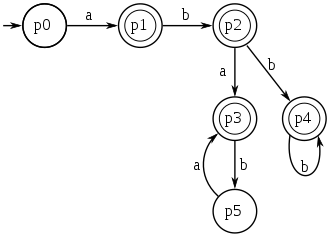
\includegraphics[width=\textwidth]{images/dfa.png}
% 		\caption{Пример графа переходов детерминированного КА.}
% 	\end{minipage}
% 	\hfill
% 	\begin{minipage}[b]{0.4\textwidth}
% 		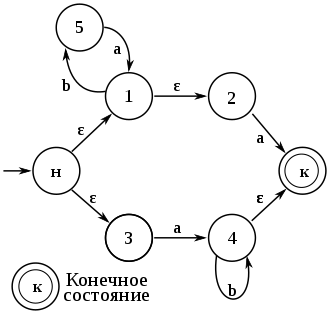
\includegraphics[width=\textwidth]{images/ndfa.png}
% 		\caption{Пример графа переходов недетерминированного КА с самопроизвольными переходами.}
% 	\end{minipage}
% \end{figure}